\documentclass[11pt]{article}
\usepackage[textwidth=18.0cm, textheight=23.0cm, top=2.0cm]{geometry}
\usepackage{pst-all}
\usepackage{amssymb}
\usepackage{tikz}
\usepackage{underscore}\begin{document}
\pagestyle{empty}


ClassName: \underline{\textbf{Class_03.2bp-8}}
\par
BinSize: \underline{\textbf{40 × 40}}
\par
ReduceSize: \underline{\textbf{40 × 40}}
\par
TypeNum: \underline{\textbf{20}}
\par
Num: \underline{\textbf{20}}
\par
OutS: \underline{\textbf{8000}}
\par
InS: \underline{\textbf{6730}}
\par
Rate: \underline{\textbf{0.841}}
\par
UB: \underline{\textbf{5}}
\par
LB0: \underline{\textbf{5}}
\par
LB: \underline{\textbf{5}}
\par
LBWithCut: \underline{\textbf{5}}
\par
NodeCut: \underline{\textbf{0}}
\par
ExtendedNodeCnt: \underline{\textbf{1}}
\par
GenNodeCnt: \underline{\textbf{1}}
\par
PrimalNode: \underline{\textbf{0}}
\par
ColumnCount: \underline{\textbf{5}}
\par
TotalCutCount: \underline{\textbf{0}}
\par
RootCutCount: \underline{\textbf{0}}
\par
LPSolverCnt: \underline{\textbf{1}}
\par
PricingSolverCnt: \underline{\textbf{0}}
\par
BranchAndBoundNum: \underline{\textbf{1}}
\par
isOpt: \underline{\textbf{true}}
\par
TimeOnPrimal: \underline{\textbf{0.000 s}}
\par
TimeOnPricing: \underline{\textbf{0.000 s}}
\par
TimeOnRmp: \underline{\textbf{0.062 s}}
\par
TotalTime: \underline{\textbf{0.125 s}}
\par
\newpage


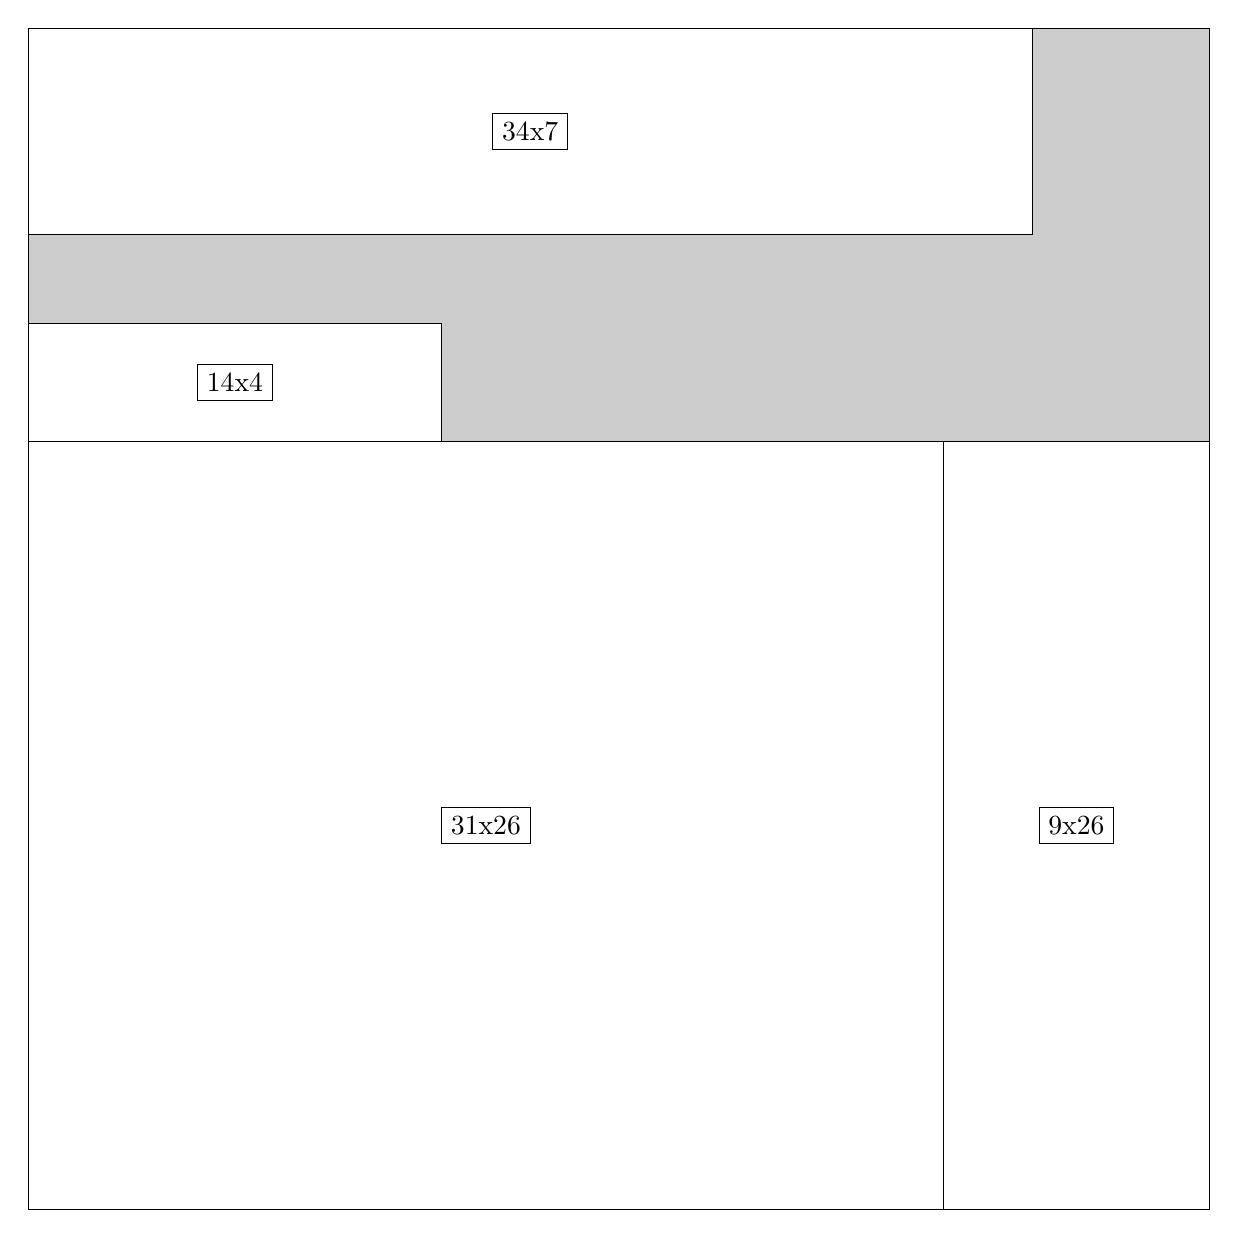
\begin{tikzpicture}[shorten >=1pt,scale=1.0,every node/.style={scale=1.0},->]
\tikzstyle{vertex}=[circle,fill=black!25,minimum size=14pt,inner sep=0pt]
\filldraw[fill=gray!40!white, draw=black] (0,0) rectangle (15.0,15.0);
\foreach \name/\x/\y/\w/\h in {31x26/0.0/0.0/11.625/9.75,14x4/0.0/9.75/5.25/1.5,34x7/0.0/12.375/12.75/2.625,9x26/11.625/0.0/3.375/9.75}
\filldraw[fill=white!40!white, draw=black] (\x,\y) rectangle node[draw] (\name) {\name} ++(\w,\h);
\end{tikzpicture}


w =31 , h =26 , x =0 , y =0 , v =806
\par
w =14 , h =4 , x =0 , y =26 , v =56
\par
w =34 , h =7 , x =0 , y =33 , v =238
\par
w =9 , h =26 , x =31 , y =0 , v =234
\par
\newpage


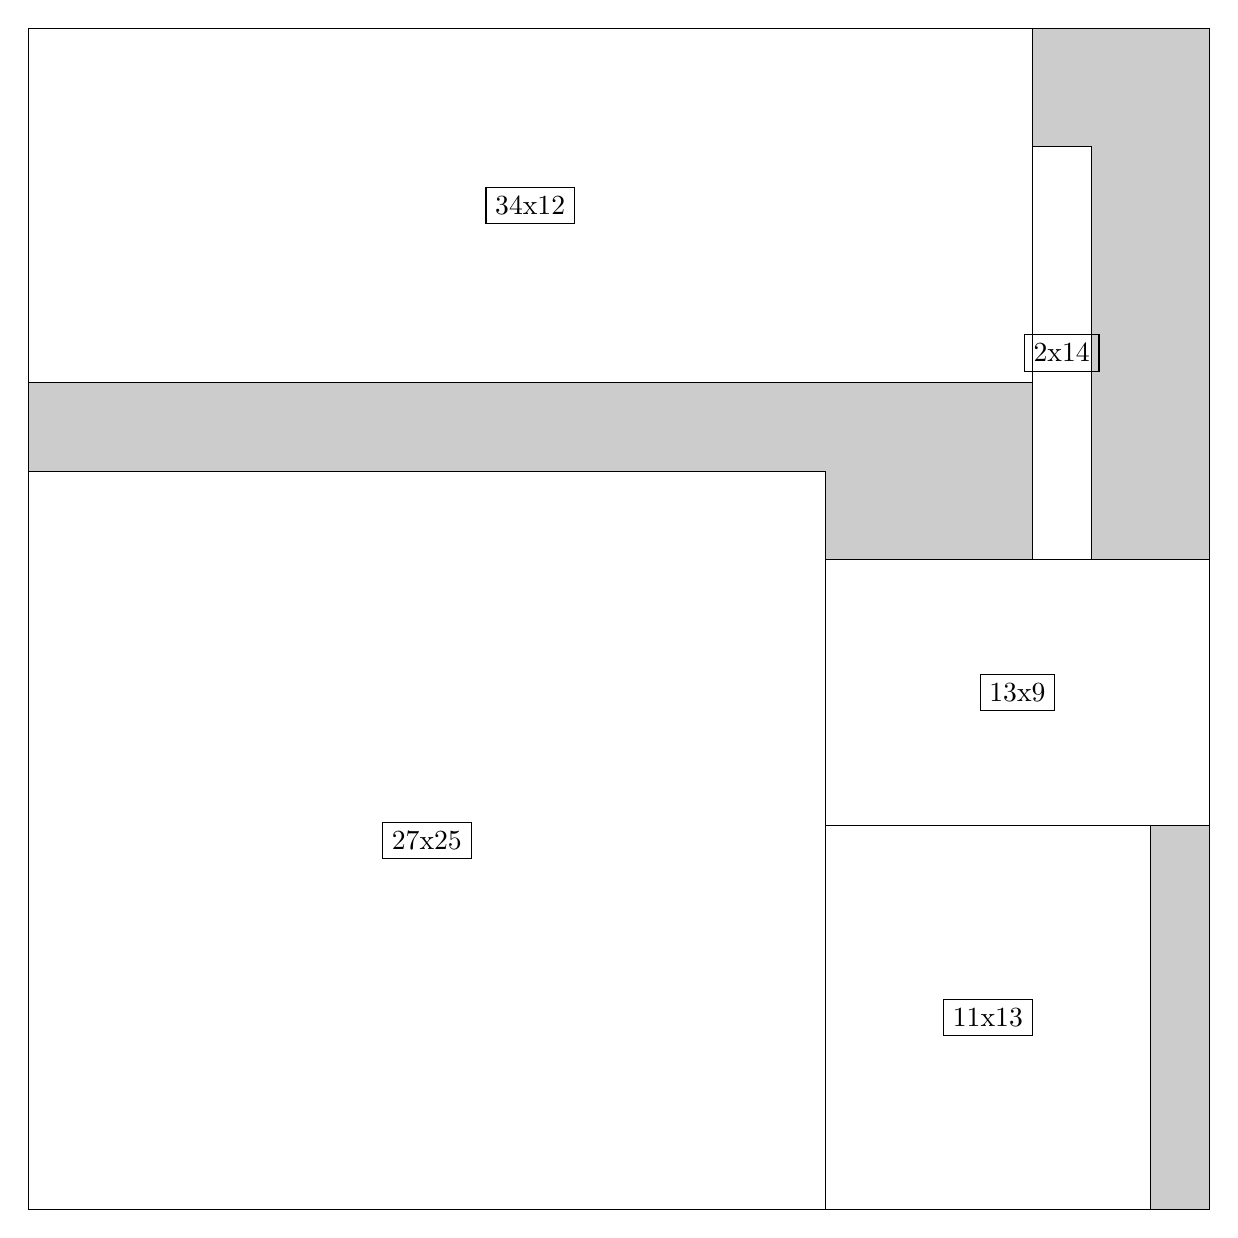
\begin{tikzpicture}[shorten >=1pt,scale=1.0,every node/.style={scale=1.0},->]
\tikzstyle{vertex}=[circle,fill=black!25,minimum size=14pt,inner sep=0pt]
\filldraw[fill=gray!40!white, draw=black] (0,0) rectangle (15.0,15.0);
\foreach \name/\x/\y/\w/\h in {11x13/10.125/0.0/4.125/4.875,27x25/0.0/0.0/10.125/9.375,34x12/0.0/10.5/12.75/4.5,13x9/10.125/4.875/4.875/3.375,2x14/12.75/8.25/0.75/5.25}
\filldraw[fill=white!40!white, draw=black] (\x,\y) rectangle node[draw] (\name) {\name} ++(\w,\h);
\end{tikzpicture}


w =11 , h =13 , x =27 , y =0 , v =143
\par
w =27 , h =25 , x =0 , y =0 , v =675
\par
w =34 , h =12 , x =0 , y =28 , v =408
\par
w =13 , h =9 , x =27 , y =13 , v =117
\par
w =2 , h =14 , x =34 , y =22 , v =28
\par
\newpage


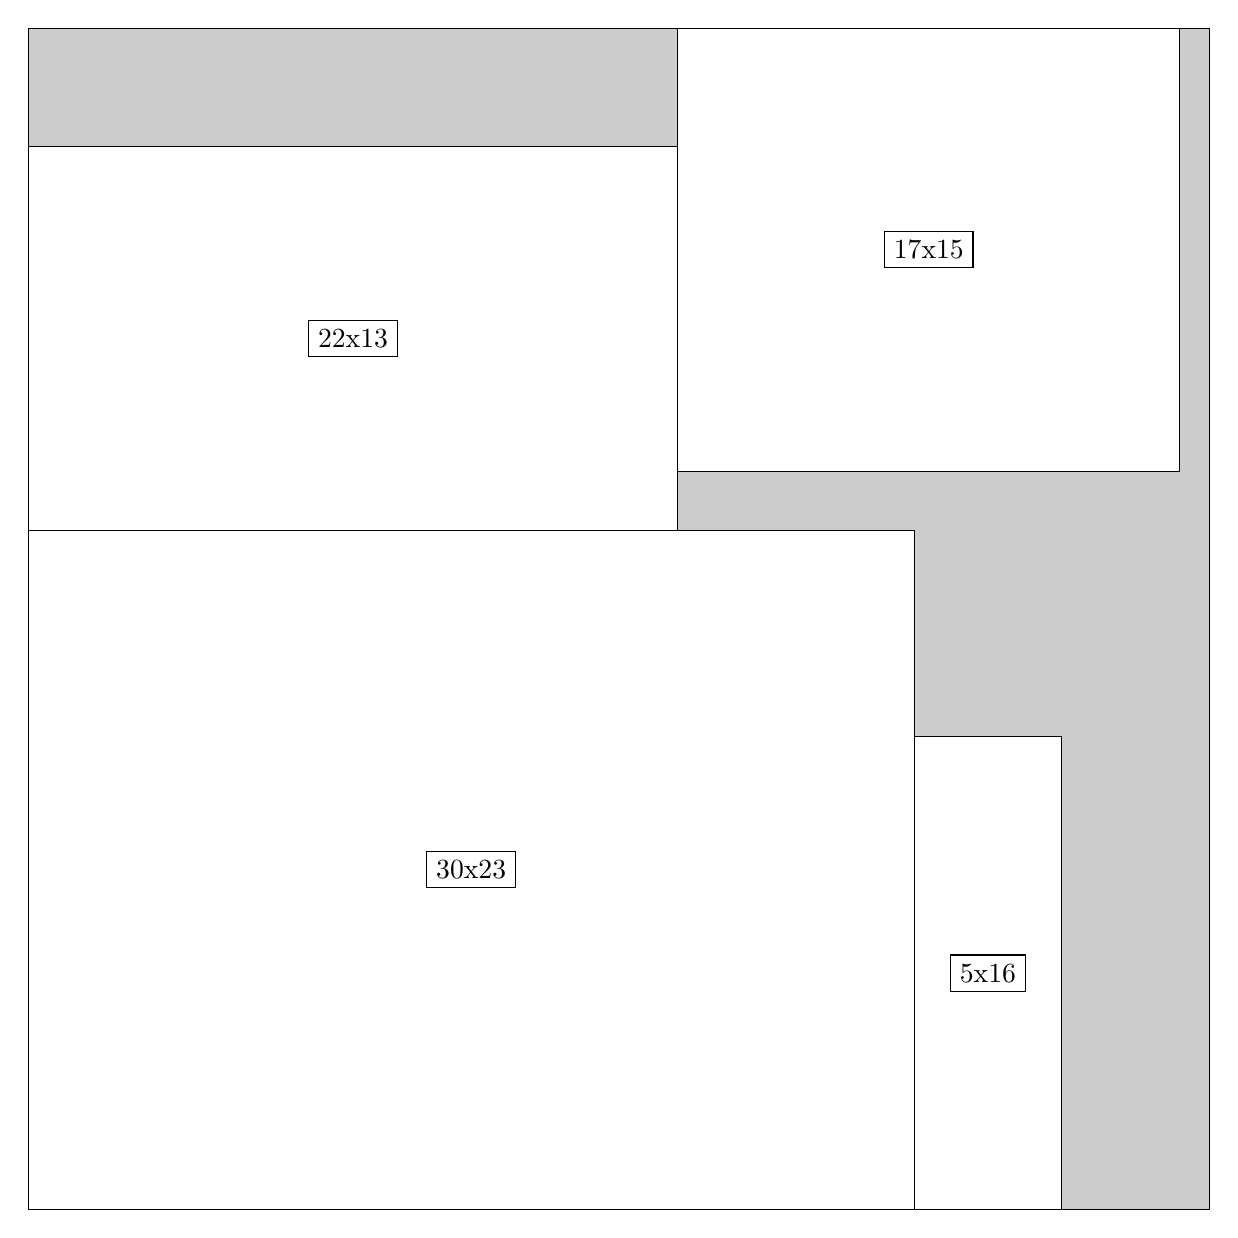
\begin{tikzpicture}[shorten >=1pt,scale=1.0,every node/.style={scale=1.0},->]
\tikzstyle{vertex}=[circle,fill=black!25,minimum size=14pt,inner sep=0pt]
\filldraw[fill=gray!40!white, draw=black] (0,0) rectangle (15.0,15.0);
\foreach \name/\x/\y/\w/\h in {22x13/0.0/8.625/8.25/4.875,17x15/8.25/9.375/6.375/5.625,30x23/0.0/0.0/11.25/8.625,5x16/11.25/0.0/1.875/6.0}
\filldraw[fill=white!40!white, draw=black] (\x,\y) rectangle node[draw] (\name) {\name} ++(\w,\h);
\end{tikzpicture}


w =22 , h =13 , x =0 , y =23 , v =286
\par
w =17 , h =15 , x =22 , y =25 , v =255
\par
w =30 , h =23 , x =0 , y =0 , v =690
\par
w =5 , h =16 , x =30 , y =0 , v =80
\par
\newpage


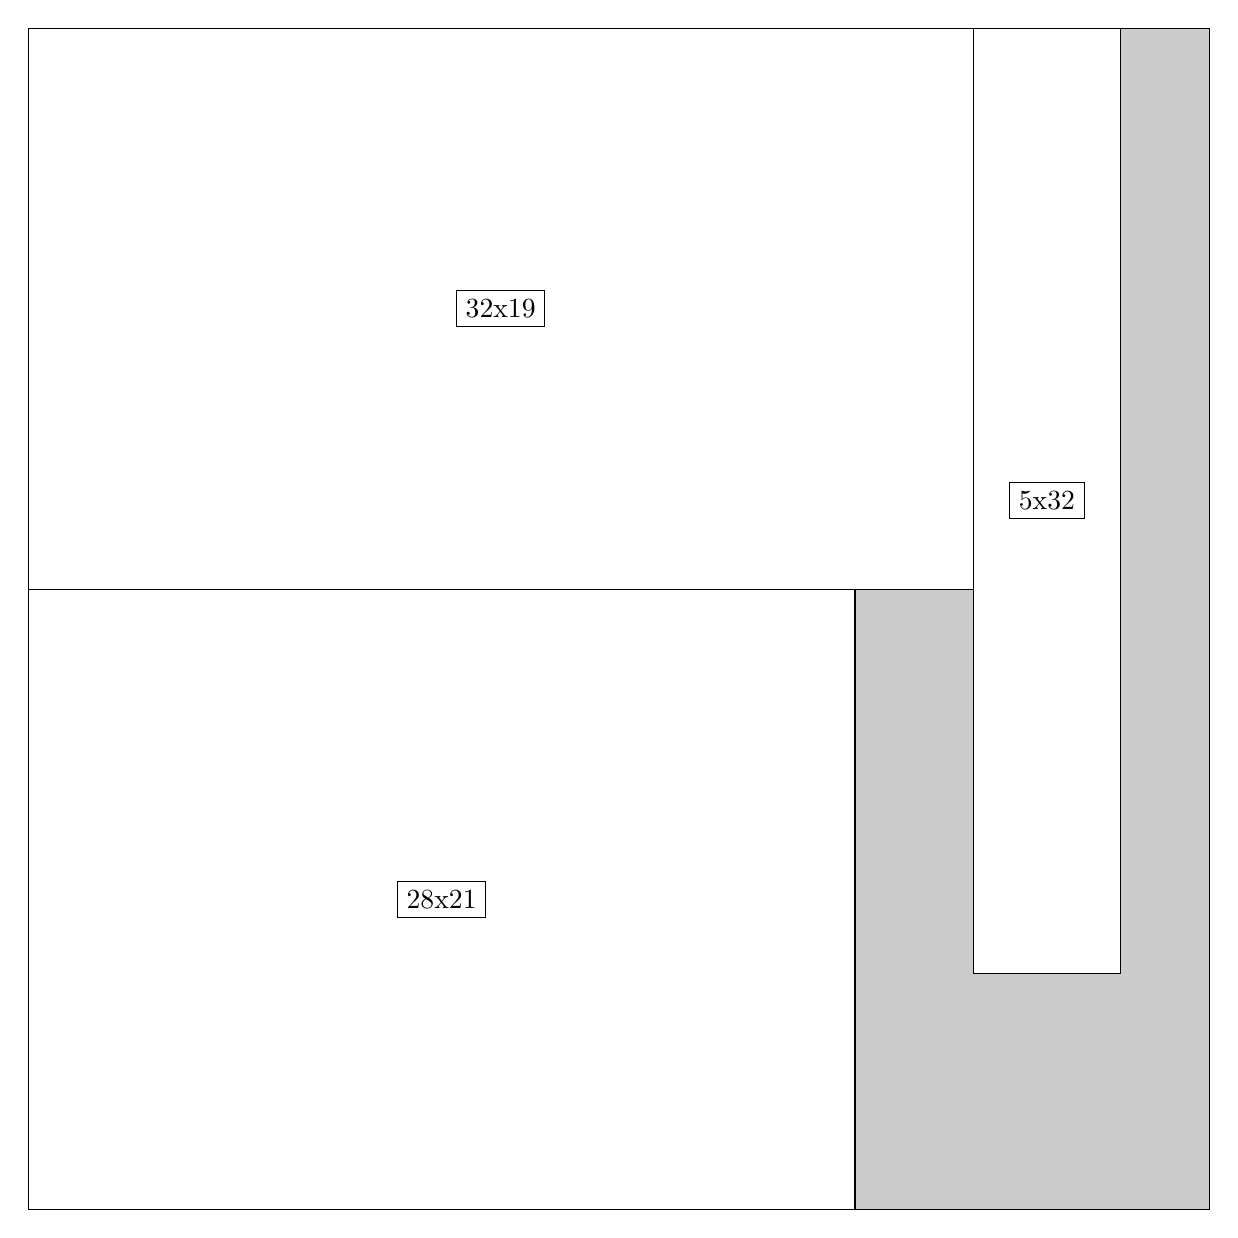
\begin{tikzpicture}[shorten >=1pt,scale=1.0,every node/.style={scale=1.0},->]
\tikzstyle{vertex}=[circle,fill=black!25,minimum size=14pt,inner sep=0pt]
\filldraw[fill=gray!40!white, draw=black] (0,0) rectangle (15.0,15.0);
\foreach \name/\x/\y/\w/\h in {32x19/0.0/7.875/12.0/7.125,5x32/12.0/3.0/1.875/12.0,28x21/0.0/0.0/10.5/7.875}
\filldraw[fill=white!40!white, draw=black] (\x,\y) rectangle node[draw] (\name) {\name} ++(\w,\h);
\end{tikzpicture}


w =32 , h =19 , x =0 , y =21 , v =608
\par
w =5 , h =32 , x =32 , y =8 , v =160
\par
w =28 , h =21 , x =0 , y =0 , v =588
\par
\newpage


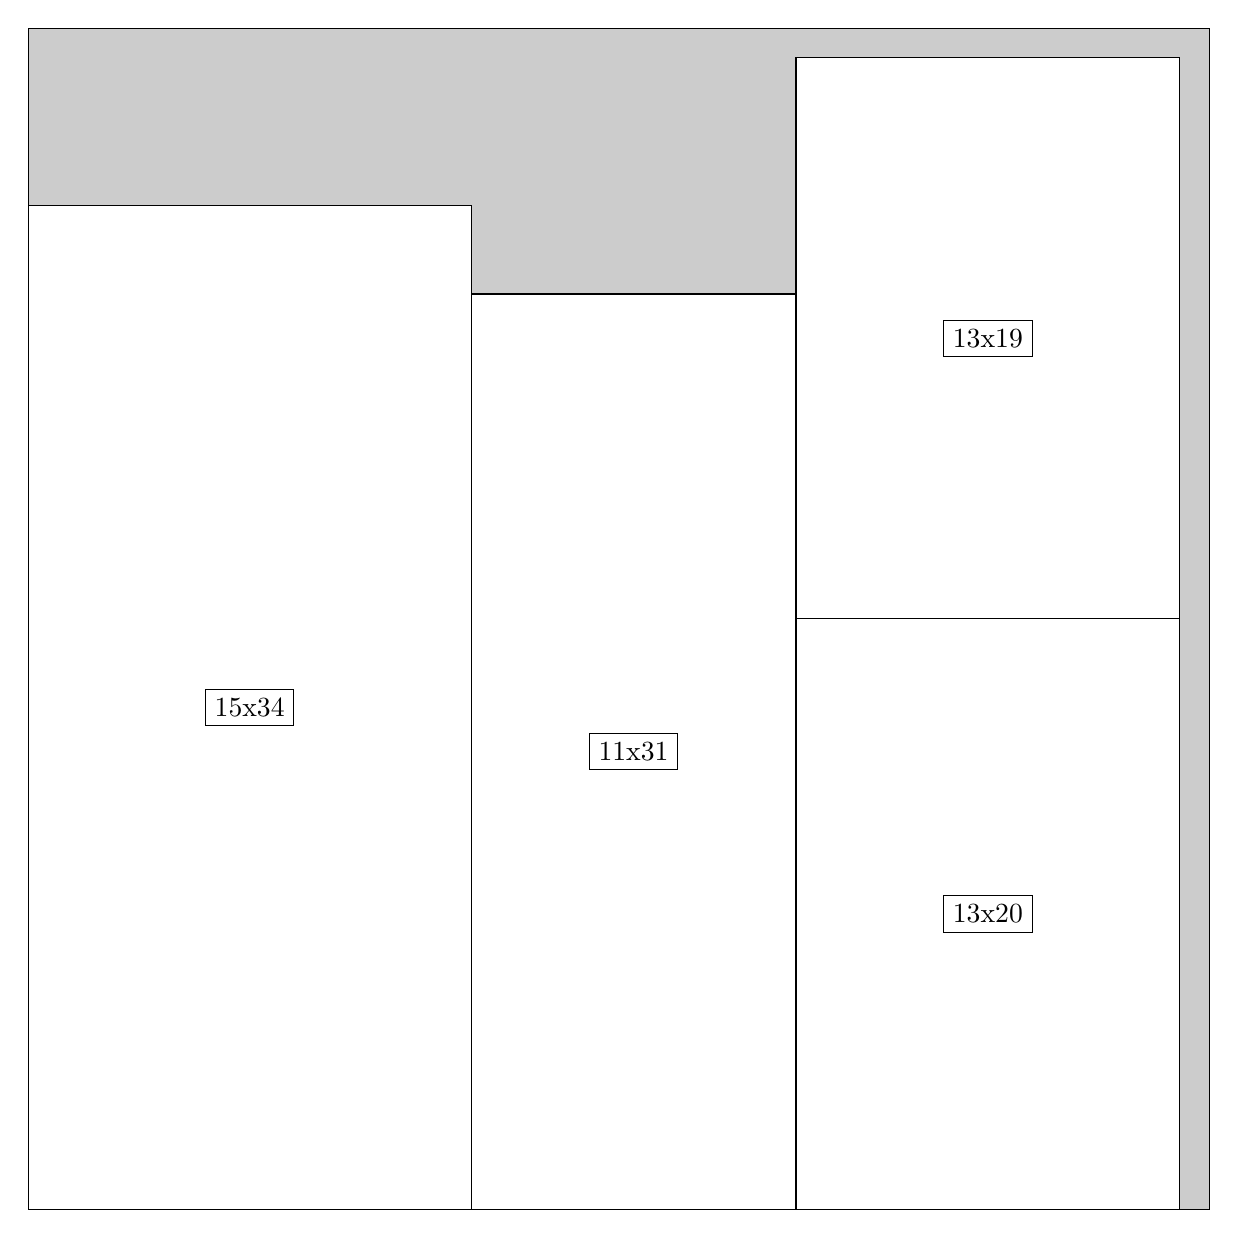
\begin{tikzpicture}[shorten >=1pt,scale=1.0,every node/.style={scale=1.0},->]
\tikzstyle{vertex}=[circle,fill=black!25,minimum size=14pt,inner sep=0pt]
\filldraw[fill=gray!40!white, draw=black] (0,0) rectangle (15.0,15.0);
\foreach \name/\x/\y/\w/\h in {15x34/0.0/0.0/5.625/12.75,11x31/5.625/0.0/4.125/11.625,13x20/9.75/0.0/4.875/7.5,13x19/9.75/7.5/4.875/7.125}
\filldraw[fill=white!40!white, draw=black] (\x,\y) rectangle node[draw] (\name) {\name} ++(\w,\h);
\end{tikzpicture}


w =15 , h =34 , x =0 , y =0 , v =510
\par
w =11 , h =31 , x =15 , y =0 , v =341
\par
w =13 , h =20 , x =26 , y =0 , v =260
\par
w =13 , h =19 , x =26 , y =20 , v =247
\par
\newpage


\end{document}